\documentclass[letterpaper]{article}
\usepackage[utf8]{inputenc}
\usepackage[spanish]{babel}
\usepackage{amssymb, amsmath}
\usepackage{graphicx}
\usepackage{lipsum}
\usepackage{dsfont}
\usepackage{vmargin}
\usepackage{setspace}
\usepackage{subcaption}
\usepackage{tocloft}
\usepackage{upgreek}
\usepackage{graphicx}

\newcommand{\fp}[1]{#1^{\prime}}
\newcommand{\de}{\dfrac{d}{dx}}

\begin{document}
	\begin{titlepage}
	    \begin{center}
	        \Large{\textbf{Tarea 02}} \\[0.1cm]
	        \huge{Matemáticas para las ciencias aplicadas I}\\[0.2cm]
	        \large{ Beristain Hernández Daniel, García Vázquez Ian Israel Merino Peña Kevin Ariel }\\
	        \today
	    \end{center}
	    \let\newpage\relax% Avoid following page break
	\end{titlepage}
\hrulefill
\section*{Continuidad}

\noindent1. Determine si las siguientes funciones son continuas en $ x_{0} $\\

a) $ f(x) = \begin{cases}
\sqrt{x^{2}-1} \text{ si } x\geq 1\\
x^{2}-2x+1, \text{ si } x \in [0,1]
\end{cases} $ en $ x_{0}=1 $

%Aquí va la respuesta

b) $ h(x) =  \begin{cases}
\dfrac{|x|}{x}, \text{  si  } x \neq 0\\
1, \text{  si  } x = 0\\
\end{cases}$ en $ x_{0} = 1 $

%Aquí va la respuesta

c) $ g(x) =  \begin{cases}
\sqrt{1-x^{2}}, \text{  si  } x \in [0,1]\\
-\sqrt{1-(x-2)^{2}}, \text{  si  } x \in [1,2]\\
\end{cases}$ en $ x_{0} = 1 $\\

%Aquí va la respuesta

\noindent2. Se inyecta una fármaco a un paciente cada 12 horas. En la Fig. 1 se muestra la concentración $ c(t) $ del fármaco en el torrente sanguíneo después de $ t $ horas.\\

a) ¿Para que valores de $ t, c(t) $ tiene discontinuidades?\\

%Aquí va la respuesta

b) ¿Qué tipo discontinuidades tiene?\\

%Aquí va la respuesta

	\begin{figure}[h!]
		\centering
		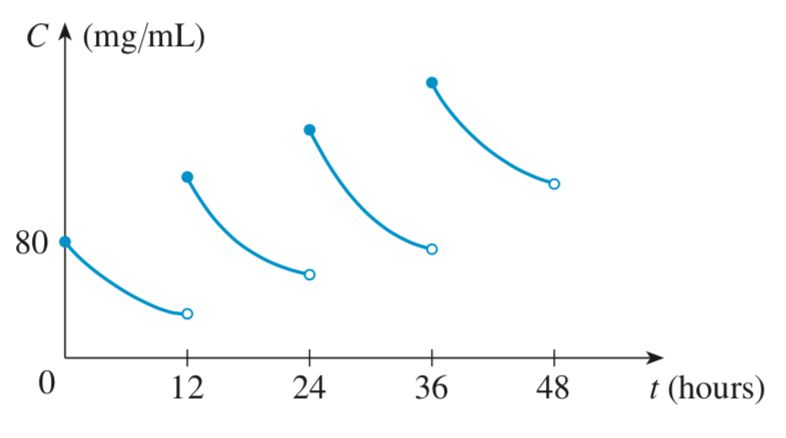
\includegraphics[scale=0.7]{img/farmaco}
		\caption{Concentración de un fármaco}
	\end{figure}

\section*{Teorema del valor intermedio}

\noindent3. Mostrar que existe algún número $ x $, tal que:\\

a) $ \sin x  = x-1$\\

%Aquí va la respuesta

b) $ x^{179}+ \dfrac{163}{1+x^{2}+\sin^{2}x} = 119 $\\
	
%Aquí va la respuesta

c) $ \cos x-\dfrac{1}{2} = x-1 $\\

%Aquí va la respuesta

d) $ (2x^{2}-2)^{2} = -x +1 $\\

%Aquí va la respuesta

\noindent4. Vea si en los siguientes incisos se cumple el teorema de valor intermedio y, en ese caso, calcule un valor intermedio.\\

a) $ f(x) = x^{3} \text{  en  } [-1,1] $\\

%Aquí va la respuesta

b) $gf(x) = x^{3} \text{  en  } [0,2] $\\

%Aquí va la respuesta

c) $ h(x) = x^{2}+4x+4 \text{  en  } [0,1] $\\

%Aquí va la respuesta

d) $ k(x) = 3x^{2} - x -1 \text{  en  } [-1,1] $\\

%Aquí va la respuesta

\noindent5. Pruebe que las ecuaciones dadas, tienen una raíz en el intervalo que se señala\\

a) $ x^{3} + 7x^{2} -3x -5 = 0$ en $ [-3.2, 0.1] $\\

%Aquí va la respuesta

b) $ x^{5} - 4x^{3} +x^{2} -1 = 0$ en $ [-2.1, 1.5] $\\

%Aquí va la respuesta

c) $ x\sin x - \dfrac{1}{2} = 0$ en $ [-1, 2] $\\

%Aquí va la respuesta

d) $ x\cos x + \dfrac{1}{2} = 0$ en $ [-1,3.5] $\\

%Aquí va la respuesta

\section*{Derivada}

\noindent6. Partiendo de la definición de derivada, mostrar que\\

a) si $ f(x) = \dfrac{1}{x}, $ entonces $ \fp{f}(a) = - \dfrac{1}{a^{2}}$ para $ a \neq 0 $\\

La derivada de una función existe si el límite $ \lim\limits_{h \to 0} \dfrac{f(x+h)-f(x)}{h} $ existe, entonces 
\begin{align*}
	& f(x) = \dfrac{1}{a} &&\text{Esta es nuestra función original}\\
	&\lim\limits_{h \to 0} \dfrac{\dfrac{1}{a+h}-\dfrac{1}{a}}{h} &&\text{Sustituyendo a por a+h}\\
	&\lim\limits_{h \to 0} \dfrac{\dfrac{a-a-h}{a(a+h)}}{h} &&\text{Operando la resta de fracciones}\\
	&\lim\limits_{h \to 0} \dfrac{-\dfrac{h}{a(a+h)}}{h} &&\text{Por el inverso aditivo de }a\\
	&\lim\limits_{h \to 0} -\dfrac{h}{ha(a+h)} &&\text{Operanddo la división de fracciones}\\
	&\lim\limits_{h \to 0} -\dfrac{1}{a(a+h)} &&\text{Por el neutro multimplicativo de }h\\
	&-\dfrac{1}{a(a+(0))} &&\text{Evaluando el límite}\\
	&-\dfrac{1}{a^{2}} \forall a \ne 0 &&\text{Evaluando el límite}\\
\end{align*}


b) si $ f(x) = \dfrac{1}{x^2}, $ entonces $ \fp{f}(a) = - \dfrac{2}{a^{3}}$ para $ a \neq 0 $\\

La derivada de una función existe si el límite $ \lim\limits_{h \to 0} \dfrac{f(x+h)-f(x)}{h} $ existe, entonces 
\begin{align*}
	& f(x) = \dfrac{1}{a^{2}} &&\text{Esta es nuestra función original}\\
	&\lim\limits_{h \to 0} \dfrac{\dfrac{1}{(a+h)^{2}}-\dfrac{1}{a^{2}}}{h} &&\text{Sustituyendo a por a+h}\\
	&\lim\limits_{h \to 0} \dfrac{\dfrac{a^{2}-(a+h)^{2}}{a^{2}(a+h)^{2}}}{h} &&\text{Operando la resta de fracciones}\\
	&\lim\limits_{h \to 0} \dfrac{\dfrac{a^{2}-a^{2}-2ah-h^{2}}{a^{2}(a+h)^{2}}}{h} &&\text{Por el inverso aditivo de }a\\
	&\lim\limits_{h \to 0} -\dfrac{h(2a+h)}{ha^{2}(a+h)^{2}} &&\text{Por el inverso aditivo de }a\\
	&\lim\limits_{h \to 0} -\dfrac{2a+h}{a^{2}(a+h)^{2}} &&\text{Por el inverso aditivo de }a\\
	&-\dfrac{2a+(0)}{a^{2}(a+(0))^{2}} &&\text{Por el inverso aditivo de }a\\
	&-\dfrac{2a}{a^{4}} &&\text{Por el inverso aditivo de }a\\
	&-\dfrac{2}{a^{3}} &&\text{Por el inverso aditivo de }a\\
\end{align*}


c) si $ f(x) = \sqrt{x}, $ entonces $ \fp{f}(a) =  \dfrac{1}{2\sqrt{a}}$ para $ a > 0 $\\

%Aquí va la respuesta

\noindent7. Encontrar la ecuación de la recta tangente en el punto $ (a, f (a)) $ para las siguientes funciones\\

a) $ f(x) = \dfrac{1}{x} $ para $ a\neq 0 $\\

%Aquí va la respuesta

b) $ f(x) = \dfrac{1}{x^{2}} $ para $ a\neq 0 $\\

%Aquí va la respuesta

c) $ f(x) = \sqrt{x} $ para $ a > 0 $\\

%Aquí va la respuesta

\noindent8. Calcular $ \fp{f}(x) $ para cada una de las siguientes funciones (sin importar los dominios de $ f y \fp{f} $).\\

a) $ f(x) = \sin(x + x^{2}) $\\

%Aquí va la respuesta

b) $ f(x) = \sin(x)+\sin(x^{2}) $\\

%Aquí va la respuesta

c) $ f(x) = \sin(\cos(x)) $\\

%Aquí va la respuesta

d) $ f(x) = \sin(\sin(x)) $\\

%Aquí va la respuesta

e) $ f(x) = \sin(x + \sin(x)) $\\

%Aquí va la respuesta

f) $ f(x) = \sin(\cos(\sin(x))) $\\

%Aquí va la respuesta

g) $ f(x) = \sin\Big(\dfrac{\cos(x)}{x}\Big) $\\

%Aquí va la respuesta

h) $ f(x) = \dfrac{\sin(\cos(x))}{x} $\\

%Aquí va la respuesta

i) $ f(x) = \dfrac{\cos(\cos(x))}{x} $\\

%Aquí va la respuesta

\section*{Teorema de Rolle}

\noindent9. Dadas las siguientes funciones, encontrar un punto que satisfaga el teorema de Rolle\\

a) $ f : [-2,0] \longrightarrow \mathds{R} $ tal que $ f(x) = x^{2} + 2x + 1 $\\

%Aquí va la respuesta

b) $ f : [0,2] \longrightarrow \mathds{R} $ tal que $ f(x) = x^{2} - 2x + 1 $\\

%Aquí va la respuesta

c) $ f : [-2,0] \longrightarrow \mathds{R} $ tal que $ f(x) = \dfrac{1}{x^{2} + 2x + 1} $\\

%Aquí va la respuesta

d) $ f : [0,2] \longrightarrow \mathds{R} $ tal que $ f(x) =\dfrac{1}{x^{2} - 2x + 1} $\\

%Aquí va la respuesta

\section*{Teorema del Valor Medio}

\noindent10. Dadas las siguientes funciones, encontrar un punto que satisfaga el teorema del Valor Medio \\

a) $ f : [-1,1] \longrightarrow \mathds{R} $ tal que $ f(x) = x^{4/3} $\\

%Aquí va la respuesta

b) $ f : [-1,2] \longrightarrow \mathds{R} $ tal que $ f(x) = x^{2} -1$\\

%Aquí va la respuesta

c) $ f : [0,2] \longrightarrow \mathds{R} $ tal que $ f(x) = x^{3} - 2x -1 $\\

%Aquí va la respuesta

d) $ f : [-2,0] \longrightarrow \mathds{R} $ tal que $ f(x) = x^{3} - 2x + 2 $\\

%Aquí va la respuesta

\section*{Regla de L’Hôpital}

\noindent11. Calcular los siguientes limites. Analice si se puede aplicar la regla de L’Hôpital\\

a)$ \lim\limits_{ x \rightarrow 0} \dfrac{x}{\tan(x)} $\\

%Aquí va la respuesta

b)$ \lim\limits_{ x \rightarrow 0} \dfrac{\cos^{2}(x) -1}{x^{2}} $\\

%Aquí va la respuesta

c)$ \lim\limits_{ x \rightarrow 0} \dfrac{b^{2}\cos(ax) -1}{x} $\\

%Aquí va la respuesta

d)$ \lim\limits_{ x \rightarrow 0} \dfrac{\sqrt{x+1} -1}{x} $\\

%Aquí va la respuesta

e)$ \lim\limits_{ x \rightarrow 1} \dfrac{2x^{2}-4x+2}{5x^{2}-10x+5} $\\

%Aquí va la respuesta

f)$ \lim\limits_{ x \rightarrow 0} \dfrac{x- \sin(x)}{x^{2}} $\\

%Aquí va la respuesta

\section*{Derivadas de funciones compuestas}

\noindent12. Para cada una de las siguientes funciones, hallar $ \fp{f} (f (x)) $.\\

a) $ f(x) = \dfrac{1}{1+x} $\\


\begin{align*}
	\fp{f}(x) &= \de \left(\frac{1}{x+1}\right)\\
	&= - \frac{1}{(x+1)^2}\\
	f'(f(x))	&= - \frac{1}{(f(x)+1)^2}\\
	&= - \frac{1}{\left(\dfrac{1}{1+x}+1\right)^2}\\
	& = - \dfrac{1}{\dfrac{1+x+1}{x+1}}\\
	& = - \dfrac{1}{\dfrac{x+2}{x+1}}\\
	& = - \dfrac{x+1}{x+2}\\
\end{align*}

b) $ f(x) = \sin(x) $\\

\begin{align*}
	f'(x) &= \de (\sin(x))\\
	&= \cos(x)\\
	&= \cos(f(x))\\
	f'(f(x))&= \cos(\sin(x))\\
\end{align*}

c) $ f(x) = x^{2} $\\

\begin{align*}
	f'(x) &= \de \left( x^2 \right)\\
	&= 2x\\
	f'(f(x)) &= 2(f(x))\\
	&= 2(x^{2})
\end{align*}

d) $ f(x) = 17 $\\

aaaaa dudaaa, en la compisición de funciones pq, según yo no se puede
\[
(f \circ g) (x) = f(g(x)) \land D_{f\circ g} = \{ x | x \in Dom_g \land g(x) \in Dom_f \}
\]

\noindent13. Para cada una de las siguientes funciones, hallar $ f(\fp{f} (x)) $.\\

a) $ f(x) = \dfrac{1}{x} $\\

\begin{align*}
	f'(x) &= \de \left( \dfrac{1}{x} \right)\\
	&= - \dfrac{1}{x^2}\\
	f(f'(x)) &= \left( \dfrac{1}{f'(x)} \right)\\
	&= \left( \dfrac{1}{- \dfrac{1}{x^2}} \right)\\
	&= -\left( \dfrac{1}{\dfrac{1}{x^2}} \right)\\
	&= x^{2}\\
\end{align*}

b) $ f(x) = x^{2} $\\

\begin{align*}
	f'(x)&= \de \left( x^{2} \right)\\
	&= 2x\\
	f(f'(x))&= (f'(x))^2\\
	&= (2x)^{2}\\
	&= 4x^{2}\\
\end{align*}

c) $ f(x) = 17x $\\

\begin{align*}
	f'(x)&= \de \left( 17x \right) \\
	&= 17\\
	f(f'(x)) &= 17(f'(x))\\
	&= 17(17)\\
	&= 17^{2}\\
\end{align*}

d) $ f(x) = 17 $\\

aaaaa dudaaa, en la compisición de funciones pq, según yo no se puede
\[
(f \circ g) (x) = f(g(x)) \land D_{f\circ g} = \{ x | x \in Dom_g \land g(x) \in Dom_f \}
\]

\noindent14. Para cada una de las siguientes funciones, hallar el máximo y el mínimo en los intervalos indicados, hallando los puntos del intervalo en que la derivada es cero y comparando los valores en estos puntos con los valores en los extremos.\\

a) $ f(x) = x^{3} -x^{2} -8x +1$ sobre $ [-2,2] $\\

%Aquí va la respuesta 

b) $ f(x) = \dfrac{x+1}{x^{2}+1}$ sobre $ [-1,\frac{1}{2}] $\\

%Aquí va la respuesta 

c) $ f(x) = x^{3} +x +1$ sobre $ [-1,1] $\\

%Aquí va la respuesta 

d) $ f(x) = \dfrac{x}{x^{2} - 1}$ sobre $ [0,5] $\\

%Aquí va la respuesta 

\section*{Interpretación geométrica de la derivada}

\noindent15. Cada una de las figuras siguientes, representan la gráfica de la derivada de una función $ f $ . Hallar todos los máximos y mínimos locales de la función $ f $ correspondiente, además diga cuando $ f $ es creciente o decreciente.\\

	\begin{figure}[ht]
		\centering
		\begin{subfigure}[l]{0.4\paperwidth}
			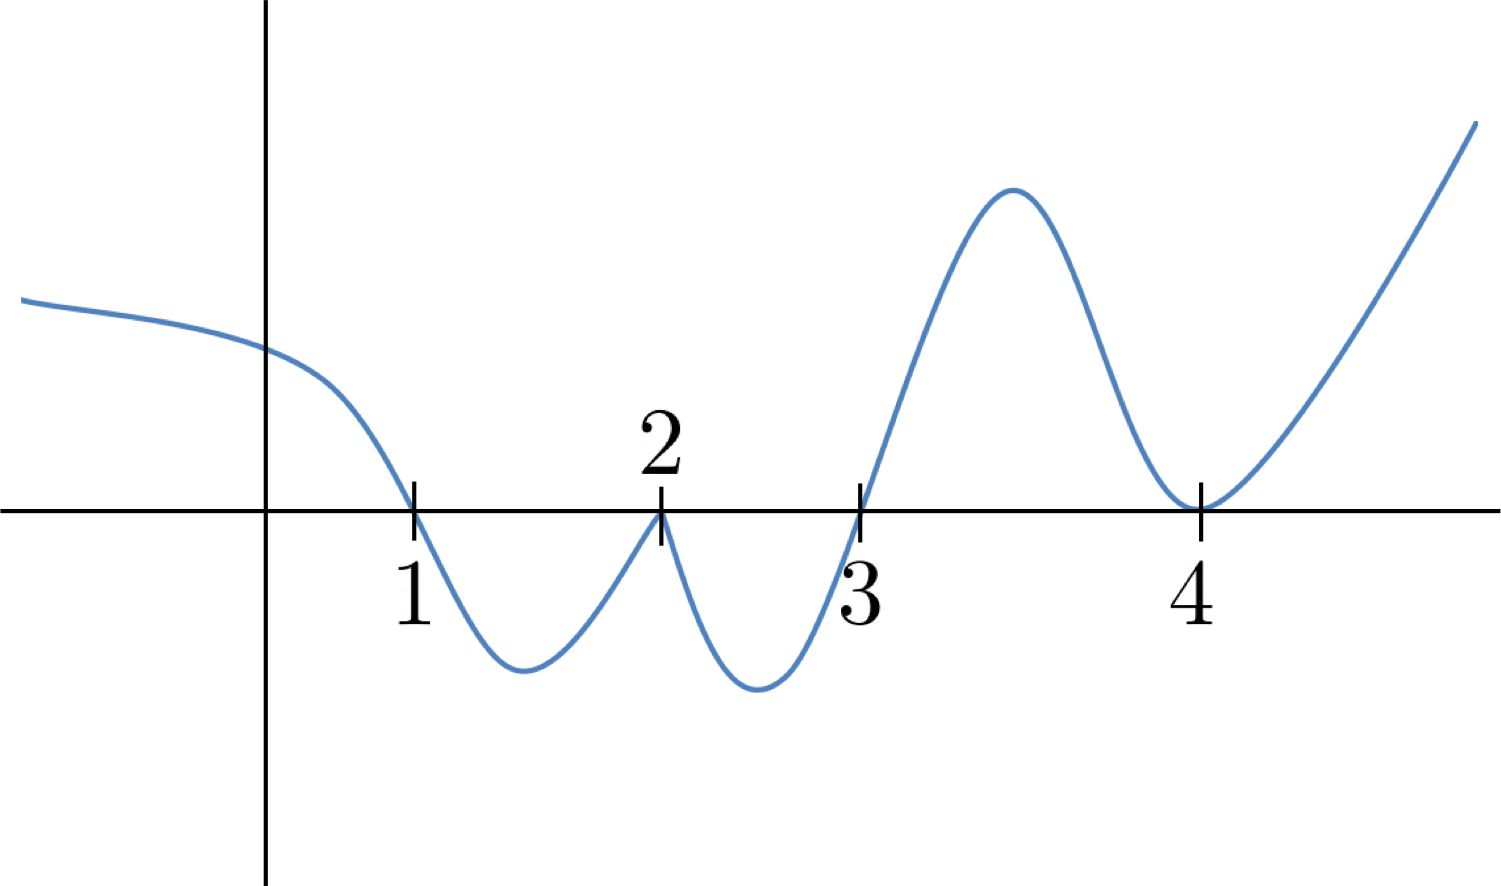
\includegraphics[scale=1]{img/imUno}
			\caption{Gráfica de la derivada de $ f $}
		\end{subfigure}
	\vspace{1cm}
		\begin{subfigure}[r]{0.4\textwidth}
			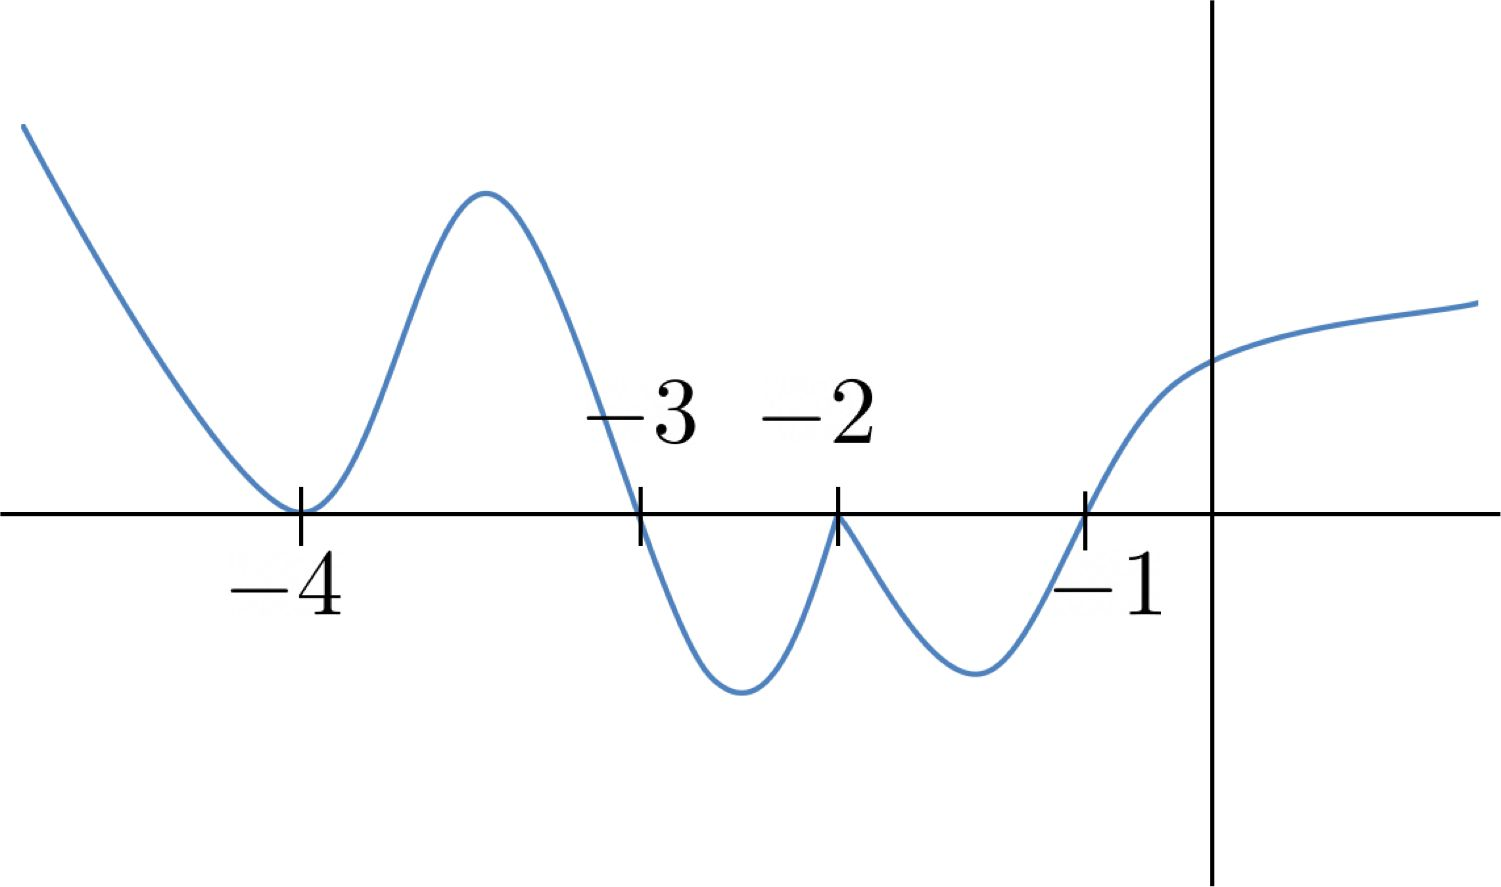
\includegraphics[scale=1]{img/imDos}
			\caption{Gráfica de la derivada de $ f $}
		\end{subfigure}
			\hspace{0.5cm}
		\begin{subfigure}[l]{0.4\paperwidth}
			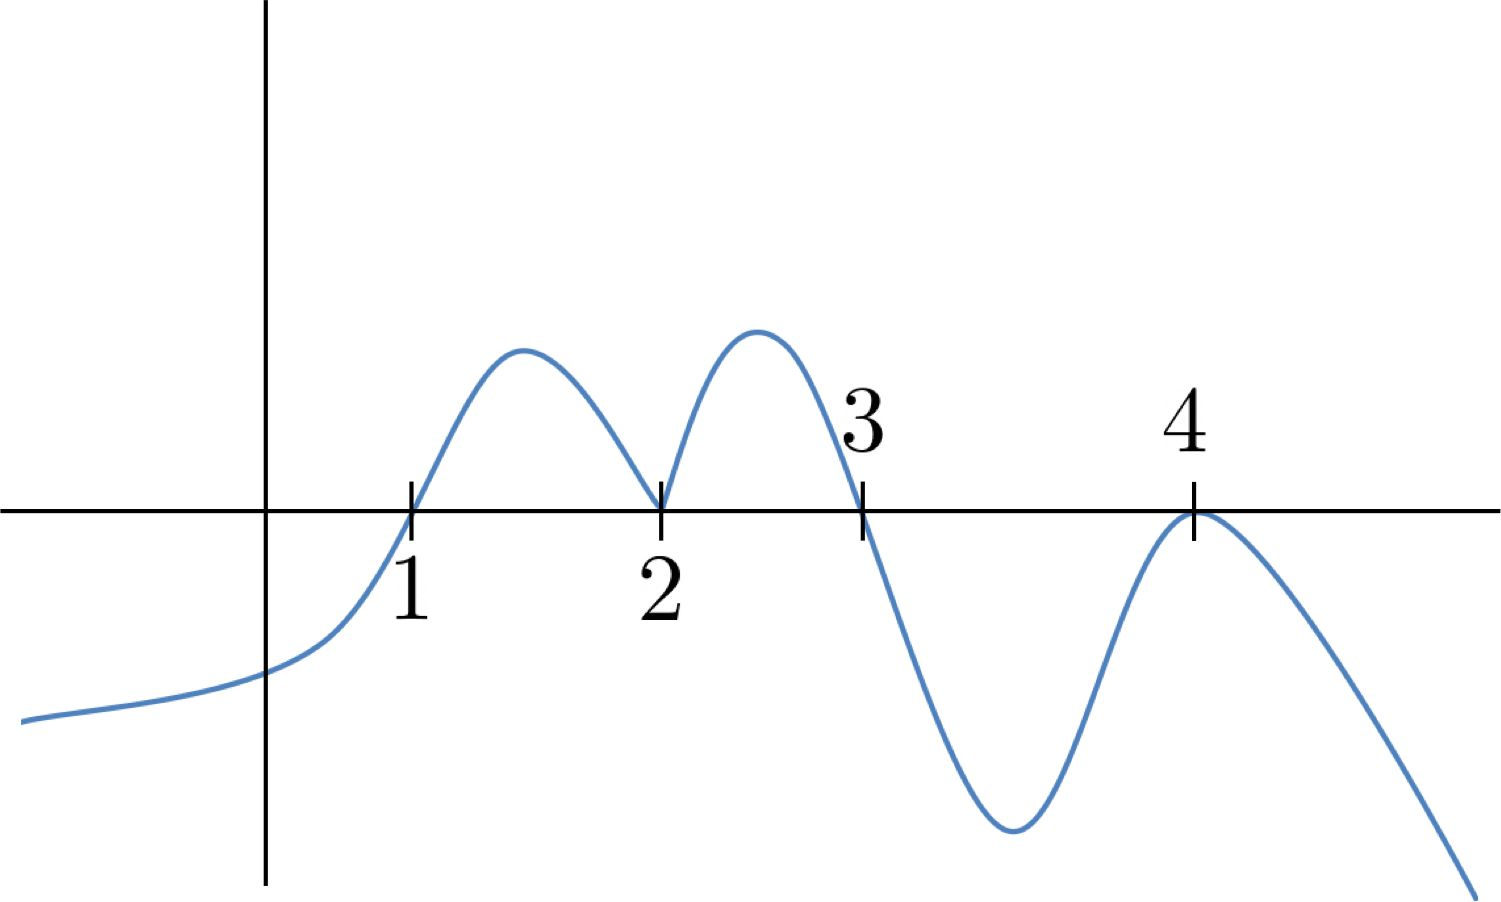
\includegraphics[scale=1]{img/imTres}
			\caption{Gráfica de la derivada de $ f $}
		\end{subfigure}
		\vspace{1cm}
		\begin{subfigure}[r]{0.4\textwidth}
			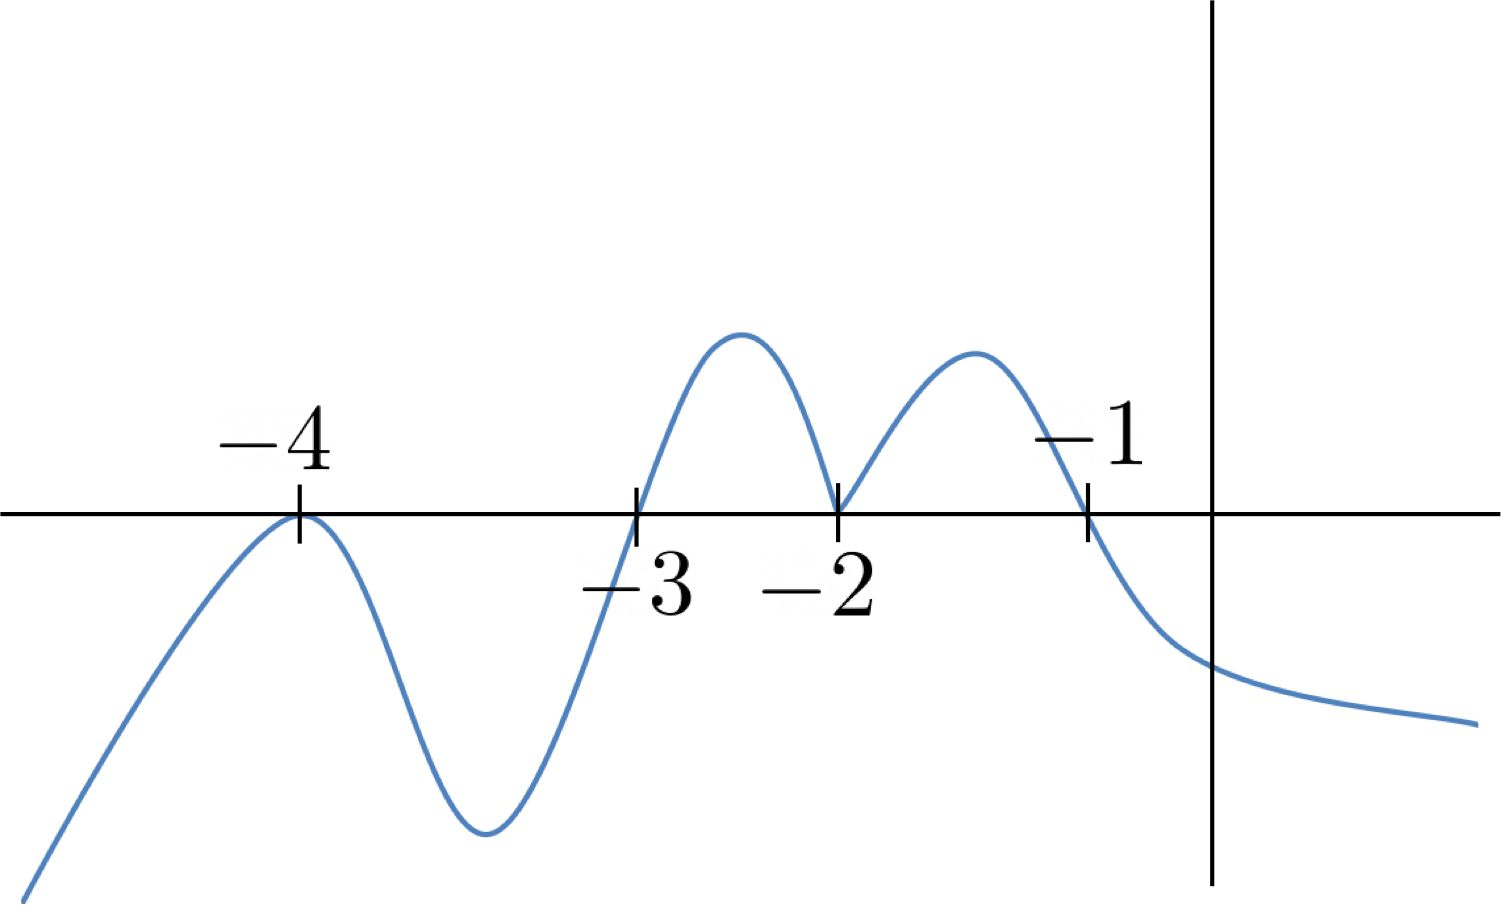
\includegraphics[scale=1]{img/imCuatro}
			\caption{Gráfica de la derivada de $ f $}
		\end{subfigure}
	\caption{ }
	\end{figure}

\noindent16. Utilizar los resultados sobre el significado de la derivada para esbozar la gráfica de las siguientes funciones (aplicar criterios de la primera y segunda derivada).\\

a) $ f(x) = x + \dfrac{1}{x} $\\

%Aquí va la respuesta

b) $ f(x) = x + \dfrac{3}{x^{2}} $\\

%Aquí va la respuesta

c) $ f(x) = \dfrac{x^{2}}{x^{2}-1} $\\

%Aquí va la respuesta

d) $ f(x) = \dfrac{1}{x^{2} + 1} $\\

%Aquí va la respuesta

\noindent 17. Mostrar que\\

a) la suma de un número real positivo y su recíproco es por lo menos 2.\\

%Aquí va la respuesta

b) Entre todos los rectángulos de igual perímetro, el de mayor área es el cuadrado.\\

%Aquí va la respuesta

c) Entre todos los rectángulos con la misma área, el cuadrado es el de perímetro mínimo.\\

%Aquí va la respuesta

d) Entre todos los rectángulos que pueden inscribirse en una circunferencia, el cuadrado es el de área máxima.\\

%Aquí va la respuesta

e) La razón de variación del volumen de una esfera respecto a su radio, es igual a su área.\\

%Aquí va la respuesta

\noindent18. Encuentre el punto para el cual\\

a) la recta tangente a la parábola $ f(x)= x^2 - 7x + 3 $, es paralela a la recta $ 5x + 3y - 3 = 0 $\\

%Aquí va la respuesta

b) la recta tangente a la parábola $ f (x) = x^2 -7x+3 $, es paralela a la recta $ 3x-y-4 =0 $\\

%Aquí va la respuesta

c) la recta tangente a la parábola $ f (x) = x^2 -7x+3 $, es paralela a la recta $ 2x + 3y - 3 = 0 $\\

%Aquí va la respuesta

\end{document}
